\documentclass[11pt]{article}
\usepackage[T1]{fontenc}
\usepackage{lmodern}
\usepackage[a4paper,margin=2.3cm]{geometry}
\usepackage{graphicx}
\usepackage{booktabs}
\usepackage{xcolor}
\usepackage{caption}
\usepackage{subcaption}
\usepackage{float}
\usepackage[hidelinks]{hyperref}

\definecolor{ink}{HTML}{1A1A1A}
\definecolor{muted}{HTML}{8A8A8A}
\definecolor{dupc}{HTML}{377EB8}
\definecolor{lossc}{HTML}{E41A1C}
\definecolor{transc}{HTML}{4DAF4A}

\captionsetup{font=small,labelfont=bf,labelsep=period}
\setlength{\parskip}{4pt}
\setlength{\parindent}{0pt}
\color{ink}

\newcommand{\EcNtips}{12}
\newcommand{\EcAge}{1}
\newcommand{\EcTreeSeed}{42}
\newcommand{\EcSimSeed}{7}
\newcommand{\EcChromLen}{4,641,652}
\newcommand{\EcRawGenes}{4506}
\newcommand{\EcGenes}{4480}
\newcommand{\EcTrimmed}{768}
\newcommand{\EcDropped}{26}
\newcommand{\EcGenicFrac}{86.8}
\newcommand{\EcBlocks}{8358}
\newcommand{\EcGeneBlocks}{4497}
\newcommand{\EcInterBlocks}{3861}
\newcommand{\EcNfamilies}{4497}
\newcommand{\EcCore}{4203}
\newcommand{\EcAccessory}{294}
\newcommand{\EcUnique}{10}
\newcommand{\EcDuplicated}{441}
\newcommand{\EcMeanGenes}{4395}
\newcommand{\EcMeanPseud}{50}
\newcommand{\EcRetention}{98.1}
\newcommand{\EcMeanSize}{4.674}
\newcommand{\EcMinGenes}{4359}
\newcommand{\EcMaxGenes}{4429}
\newcommand{\EcDup}{474}
\newcommand{\EcTrans}{496}
\newcommand{\EcLoss}{788}
\newcommand{\EcPseudo}{330}
\newcommand{\EcInv}{134}
\newcommand{\EcTransp}{47}
\newcommand{\EcOrig}{18}
\newcommand{\EcInvR}{4e-06}
\newcommand{\EcLossR}{7e-06}
\newcommand{\EcDupR}{3e-06}
\newcommand{\EcTransR}{3e-06}
\newcommand{\EcTranspR}{2e-06}
\newcommand{\EcOrigR}{2}
\newcommand{\EcExt}{0.9996}
\newcommand{\EcMeanEvLen}{2,500}
\newcommand{\EcPseudoP}{0.4}
\newcommand{\EcReplP}{0.4}
\newcommand{\EcExampleGene}{b2876}


\title{\vspace{-1.2cm}\textbf{Evolving a real bacterial genome with ZOMBI2's\\
nucleotide model}\\[2pt]
\large The \textit{Escherichia coli} K-12 chromosome along a simulated 12-species tree}
\author{ZOMBI2 --- nucleotide genic model}
\date{}

\begin{document}
\maketitle
\vspace{-0.8cm}

\begin{abstract}\noindent
We take the real annotation of \textit{Escherichia coli} K-12 MG1655 --- a single circular
chromosome of \EcChromLen~bp carrying \EcGenes~genes --- as the ancestral genome, and evolve it
forward along a simulated \EcNtips-species tree with ZOMBI2's \emph{nucleotide genic} model. Genes
are never broken by structural events; losses may pseudogenise a gene instead of deleting it, and
transfers may replace a recipient's homologous locus. From one run we recover a full pan-genome:
\EcCore~core and \EcAccessory~accessory gene families, \EcDuplicated~families with paralogs, and a
reconstructed gene tree for every gene and intergene. This is a worked demonstration that the model
scales to a megabase-sized real genome and reproduces textbook bacterial genome dynamics.
\end{abstract}

\section{Model and set-up}

\textbf{The ancestral genome.} We read the RefSeq GFF3 of \textit{E.\ coli} K-12 MG1655
(assembly \texttt{GCF\_000005845.2}, chromosome \texttt{NC\_000913.3}). ZOMBI2 copies the
chromosome length (\EcChromLen~bp, circular) and the coordinates of its genes; the intergenic
regions are simply the gaps between them. Bacterial genes overlap (shared start/stop codons, nested
ORFs), and the genic model forbids event breakpoints \emph{inside} a gene, so overlaps are removed by
trimming: of \EcRawGenes~annotated genes, \EcTrimmed~had their start clipped to the previous gene's
end and \EcDropped~nested genes were dropped, leaving \EcGenes~disjoint genes covering
\EcGenicFrac\,\% of the chromosome.

\textbf{The species tree.} A \EcNtips-tip tree (Fig.~\ref{fig:tree}) was simulated under a
birth--death process ($\lambda=1.0$, $\mu=0.35$, crown age \EcAge; seed \EcTreeSeed).

\textbf{The evolutionary model.} Genes and intergenes evolve by variable-length structural events
whose rates are \emph{per nucleotide}: inversion \EcInvR, loss \EcLossR, duplication \EcDupR,
transfer \EcTransR{} and transposition \EcTranspR{} per site, plus origination \EcOrigR{} per branch.
Event lengths are geometric with mean \EcMeanEvLen~bp (extension \EcExt). A loss that hits a gene
pseudogenises it --- keeping the sequence but marking it non-functional --- with probability
\EcPseudoP; a transfer is a homologous replacement with probability \EcReplP{} (seed \EcSimSeed).

Because genes are never cut, each of the \EcGenes~genes stays a single indivisible unit (an
\emph{block}) wherever it survives, while intergenic DNA fragments freely. The run yields
\EcBlocks~blocks in total: \EcGeneBlocks~gene blocks (the \EcGenes~ancestral genes plus \EcOrig{}
originated \emph{de novo}) and \EcInterBlocks~intergene blocks.

\begin{figure}[H]
\centering
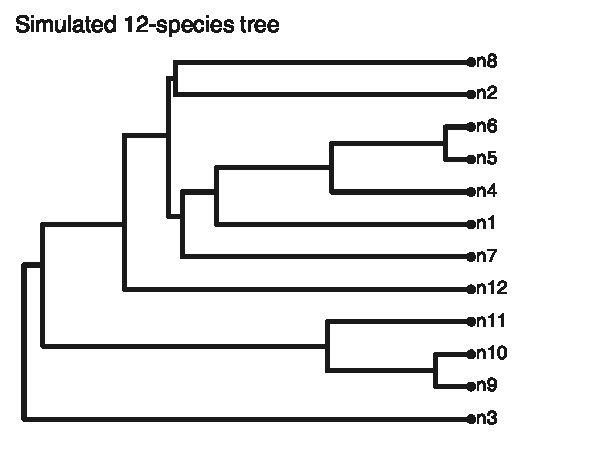
\includegraphics[width=0.62\textwidth]{figs/fig1_species_tree.pdf}
\caption{The simulated \EcNtips-species tree the genome was evolved along.}
\label{fig:tree}
\end{figure}

\section{Results}

\subsection{Genome dynamics along the tree}

Every lineage erodes and innovates (Fig.~\ref{fig:dynamics}). Averaged over the \EcNtips~extant
genomes, \EcRetention\,\% of the ancestral genes are retained (mean \EcMeanGenes~genes; range
\EcMinGenes--\EcMaxGenes) at a mean genome size of \EcMeanSize~Mbp, with \EcMeanPseud~pseudogenes per
genome. Gene loss (\textcolor{lossc}{red}) and pseudogenisation dominate the erosion side; gene
duplication (\textcolor{dupc}{blue}) and the occasional \emph{de novo} origination
(\textcolor{transc}{green}) drive innovation.

\begin{figure}[H]
\centering
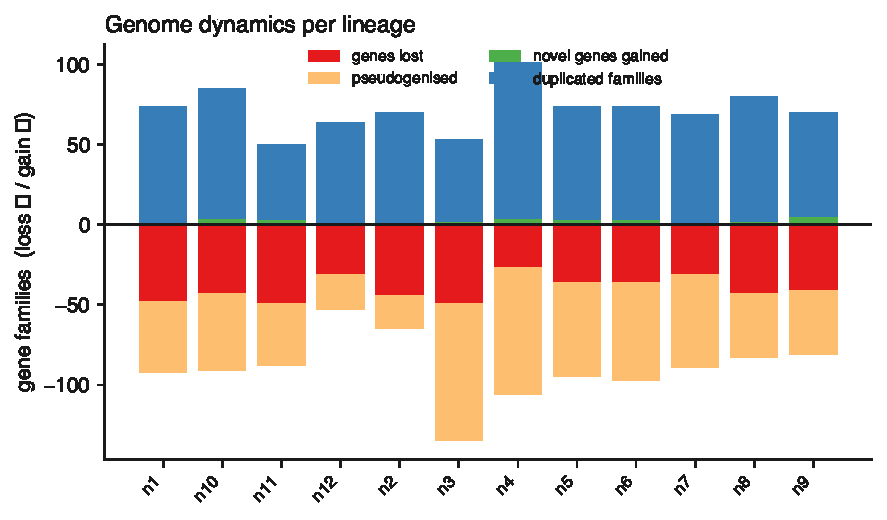
\includegraphics[width=0.80\textwidth]{figs/fig2_gene_content.pdf}
\caption{Per-lineage genome dynamics relative to the ancestral \textit{E.\ coli} gene set:
genes lost and pseudogenised (below the axis) versus novel genes gained and families duplicated
(above). Each lineage has its own history of gain and loss.}
\label{fig:dynamics}
\end{figure}

\subsection{A pan-genome emerges}

Reading gene presence across the \EcNtips~genomes gives the classic bacterial pan-genome
(Fig.~\ref{fig:pan}, left): a large \textbf{core} of \EcCore~families present in every species, a
long \textbf{accessory} tail of \EcAccessory~families (\EcUnique~found in a single genome), produced
purely by lineage-specific loss, transfer and origination. \EcDuplicated~families carry paralogs in
at least one genome. The copy-number matrix of the most variable families
(Fig.~\ref{fig:pan}, right) shows the gains (dark), single copies (salmon) and losses (pale) that
make up this variation.

\begin{figure}[H]
\centering
\begin{subfigure}{0.44\textwidth}
  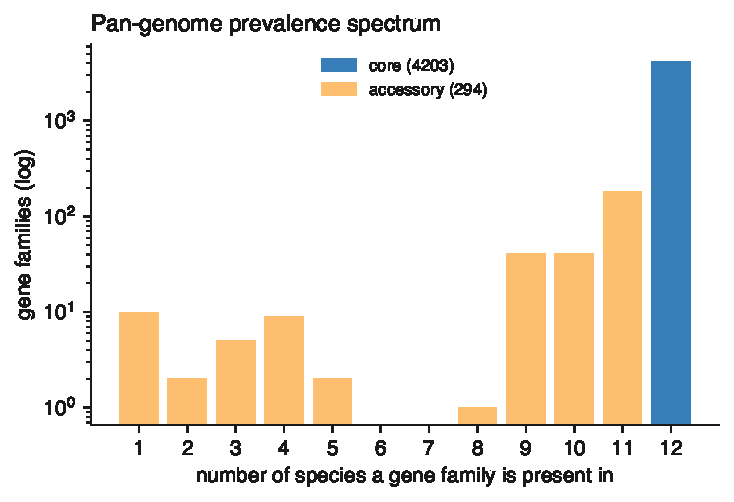
\includegraphics[width=\textwidth]{figs/fig3_pangenome.pdf}
\end{subfigure}\hfill
\begin{subfigure}{0.53\textwidth}
  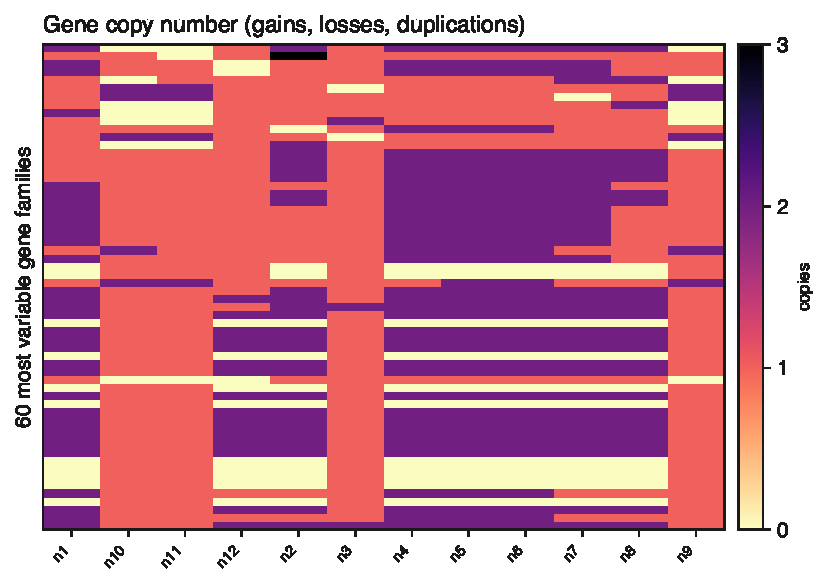
\includegraphics[width=\textwidth]{figs/fig4_heatmap.pdf}
\end{subfigure}
\caption{\textbf{Left:} pan-genome prevalence spectrum (log scale) --- the U-shaped core/accessory
split. \textbf{Right:} copy number of the 60 most variable gene families across the \EcNtips~genomes.}
\label{fig:pan}
\end{figure}

\subsection{The events behind it, and gene-tree discordance}

The whole history is one event log (Fig.~\ref{fig:genetree}, left): \EcLoss~losses, \EcPseudo{}
pseudogenisations, \EcDup~duplications, \EcTrans~transfers, \EcInv~inversions,
\EcTransp~transpositions and \EcOrig~originations. Because the model re-mints lineages at every
event, ZOMBI2 reconstructs a gene tree for each gene block. Duplications and transfers make these gene
trees disagree with the species tree: Fig.~\ref{fig:genetree} contrasts the species tree with the
reconstructed tree of gene \texttt{\EcExampleGene}, whose duplication history gives it several
paralogous copies per lineage --- a topology no strictly-vertical model could produce.

\begin{figure}[H]
\centering
\begin{subfigure}{0.42\textwidth}
  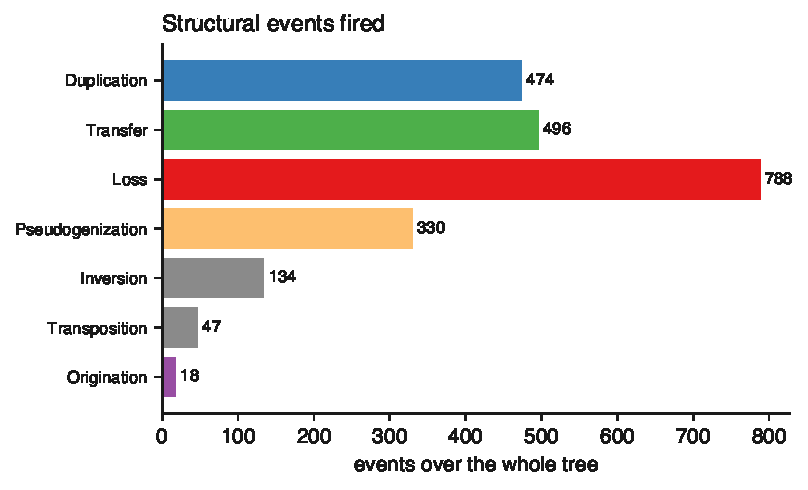
\includegraphics[width=\textwidth]{figs/fig5_events.pdf}
\end{subfigure}\hfill
\begin{subfigure}{0.55\textwidth}
  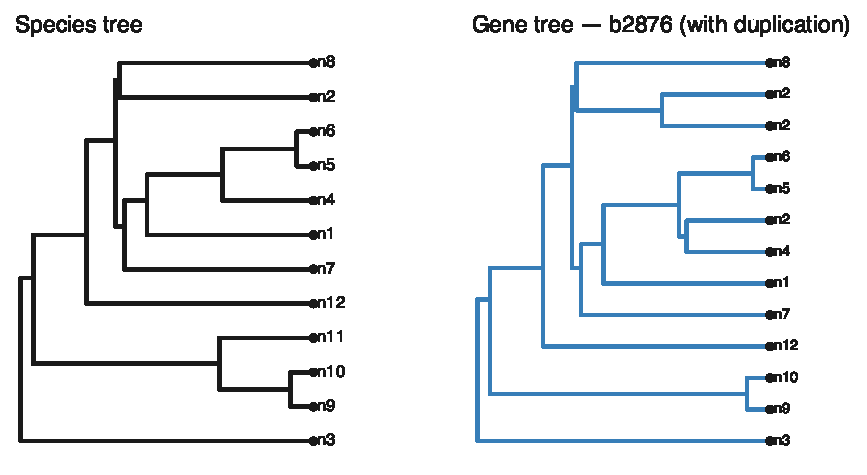
\includegraphics[width=\textwidth]{figs/fig6_genetree.pdf}
\end{subfigure}
\caption{\textbf{Left:} structural events fired over the whole tree. \textbf{Right:} the species
tree beside the reconstructed gene tree of \texttt{\EcExampleGene} --- paralogs from duplication make
the gene tree discordant.}
\label{fig:genetree}
\end{figure}

\section{Summary}

Starting from nothing but a GFF file and a tree, ZOMBI2's nucleotide genic model evolves a real
\EcChromLen~bp bacterial chromosome and delivers, in one self-consistent run: extant genomes with
realistic sizes, a core/accessory pan-genome, gene duplications and transfers, pseudogenisation, and
a ground-truth gene tree for every gene and intergene. Every gene stays intact throughout, so the
output can be read as a known-truth benchmark for pan-genome, orthology and gene-tree/species-tree
reconciliation methods on genomes with authentic architecture. The full run takes under a second.

\vfill
{\footnotesize\color{muted}Reproduce with \texttt{python run\_analysis.py} in
\texttt{ecoli\_nt\_analysis/} (tree seed \EcTreeSeed, simulation seed \EcSimSeed). Generated with
ZOMBI2 \texttt{zombi2 genomes --rate-model nucleotide --gff}.}

\end{document}
